\subsection{Four stable slices in exterior coordinates}
\label{sec:exterior-zipper-atlas}

The comparative figures use DD$(1,0)$, DD$(1,1)$, DO$(1,0)$ and
DO$(1,1)$. The first DD signature represents the reflected pair
$01,10$; retaining one of them makes the four-family comparison more
direct. Each displayed region is a subset of a two-real-dimensional
zipper surface in an ambient four-real-dimensional parameter space.
The following exterior coordinates place these surfaces in a common
geometric display while keeping the fourth coordinate explicit.

For canonical coefficients $(a,b)$, put
\begin{equation}\label{eq:exterior-canonical-coefficients}
 c_1=1/a,\qquad c_2=1/b.
\end{equation}
The strict contraction domain is exactly $|c_1|>1$, $|c_2|>1$.
These are reciprocal coefficients; if a generator is opposite, its
inverse map is $S_j^{-1}(z)=J_{\kappa_j}(c_j(z-t_j))$, with
$t_1=-1,t_2=1$. In particular, the conjugation remains part of the
inverse map.

It is useful to distinguish this canonical pair from the unsigned
endpoint coordinates
\begin{equation}\label{eq:exterior-endpoint-coordinates}
 c=\frac1q,\qquad v=\frac1{1-q}=\frac{c}{c-1},\qquad
 (c-1)(v-1)=1.
\end{equation}
The contraction lens becomes $|c|>1$, $\Re c>1/2$, and the common
necessary condition for stability becomes the half-plane $\Re c>1$.
Thus the reciprocal chart makes the stable-set bound linear. The
planar panels below use this $c$ coordinate. For all four selected
families the canonical first coefficient is instead $c_1=-c$.

\begin{proposition}[Exterior placement of the four selected surfaces]
\label{prop:four-exterior-surfaces}
Write $q=x+iy$, $s=|q|^2$, and set
\[
 N_{10}=3x-2y^2+iy(2x-1),\qquad
 N_{11}=1+q+s(2q-1).
\]
Both quantities are nonzero throughout $\Omega$. For the selected
signatures $e=(1,e_2)$, the canonical exterior coefficients are
\begin{equation}\label{eq:four-exterior-surfaces}
\begin{array}{c|cc}
\text{plane type}&c_1&c_2\\\hline
\mathrm{DD}&-c&(-1)^{e_2}v\\[2pt]
\mathrm{DO}&-c&(-1)^{e_2}v\,N_{1e_2}/\overline{N_{1e_2}}.
\end{array}
\end{equation}
Consequently the DO surfaces include a nonconstant phase rotation of
the opposite coefficient. Their endpoint equations alone do not give
their placement in the canonical coefficient chart.
\end{proposition}
\begin{proof}
Direct coefficients are unchanged by complex-affine conjugacy, giving
the DD row. For DO, the first endpoint map is $F_1(z)=q-qz$ and the
second has coefficient $B=(-1)^{e_2}(1-q)$ multiplying $\overline z$.
Put $D=3(1+2x)$. Solving for the fixed point $m$ of
$(F_1+F_2)/2$ gives
\[
 m_{10}=\frac{4q+2\overline q}{D},\qquad
 m_{11}=\frac{1+3q+2s}{D}.
\]
The normalizing displacement in
Proposition~\ref{prop:canonical-normalization} is
$d=F_2(m)-m=m-F_1(m)=(1+q)m-q=N_{1e_2}/D$.
Hence $a=-q$ and $b=B\overline d/d=B\overline N/N$, proving
the formula after reciprocation. The lens has $0<x<1$, so $D>0$.
If $N_{10}=0$, its imaginary part forces either $y=0$ or $x=1/2$.
In the first case its real part is $3x>0$; in the second it is
$3/2-2y^2>0$ because $y^2<3/4$. Finally,
$\Re N_{11}=1-s+x(1+2s)>0$, since $s<1$ and $x>0$.
\end{proof}

\paragraph{Projection of the four-dimensional atlas.}
Use the canonical coefficient phases
\[
 \theta_1=\arg a=\alpha-\gamma,\qquad
 \theta_2=\arg b=-\alpha-\gamma
 \pmod{2\pi}.
\]
Together with
\begin{equation}\label{eq:exterior-weight-radial}
 w=\frac{|c_2|}{|c_1|+|c_2|},\qquad
 \rho=\frac{2|c_1||c_2|}{|c_1|+|c_2|},
\end{equation}
these give four real coordinates. Define
\begin{equation}\label{eq:zipper-three-dimensional-projection}
\begin{split}
 X&=(4+\rho\cos\theta_1)\cos\theta_2,\\
 Y&=(4+\rho\cos\theta_1)\sin\theta_2,\\
 Z&=\rho\sin\theta_1.
\end{split}
\end{equation}
This map respects the phase lattice~\eqref{eq:phase-lattice}. At any
fixed $w$, it is injective on the connectedness range $0<\rho\le2$:
if $R=\sqrt{X^2+Y^2}$, then
\[
 \rho=\sqrt{(R-4)^2+Z^2},\quad
 \theta_1=\arg(R-4+iZ),\quad
 \theta_2=\arg(X+iY).
\]
Across different weights the display omits one coordinate. Colour
records $w$, so the projected position together with its numerical
weight recovers the exterior pair
\[
 c_1=\frac{\rho}{2w}e^{-i\theta_1},\qquad
 c_2=\frac{\rho}{2(1-w)}e^{-i\theta_2}.
\]
Projected overlaps at distinct weights do not assert intersections
in four dimensions. DD and DO remain separate discrete orientation
classes and are displayed separately.

On every zipper surface,
$w=|q|/(|q|+|1-q|)$ and $\rho=2/(|q|+|1-q|)$. Its stable set lies in
\begin{equation}\label{eq:exterior-stable-band}
 2\sqrt{w^2+(1-w)^2}<\rho\le2.
\end{equation}
The wireframe $\rho=2$ in Figure~\ref{fig:zipper-stable-atlas} is an
outer coordinate reference. It is not a computed connectedness
boundary. The central opening is imposed by the toroidal projection.

\paragraph{Certified stable regions and linked curve probes.}
The coloured surfaces and planar regions are images of closed parameter
cells certified by Proposition~\ref{prop:zipper-return-certificate}.
Their union is a finite inner cover of the stable set. The figures
show this positive evidence without assigning a membership class to
the unpainted part of the plane or the projection. In particular,
an apparent gap between cells is not a proved barrier, and the edge
of the displayed cover need not be a stable-set boundary. Curved
images of cells are drawn by a finite mesh; the underlying
certificate is attached to the original $q$ cell. The exterior panels
show the finite window $0.96\le\Re c\le4.65$,
$-2.70\le\Im c\le0.13$. Their lower half corresponds to
$\Im q\ge0$; conjugation gives the other half. The unbounded
tail as $q\to0$ continues beyond the window.

The same three endpoint parameters link each selected family to
three planar curve examples:
\begin{equation}\label{eq:three-shared-zipper-probes}
 q_A=\tfrac12+\tfrac15i,\qquad
 q_B=\tfrac12+\tfrac25i,\qquad
 q_C=L=\frac{272727+347877i}{800000}.
\end{equation}
The parameters $q_A,q_B$ are certified stable in all four families.
At $q_C$, DD$(1,1)$ and DO$(1,1)$ are certified stable. The DD case
is the point in Calegari's disconnected wiggle locus. At the same
endpoint parameter, DO$(1,0)$ has an additional identification,
certified by the exact degree calculation described in
Appendix~\ref{app:zipper-computation}. The present certificates do
not classify DD$(1,0)$ at $q_C$. The three examples therefore compare
the geometry of the four marked families at common parameters;
they do not assert that all twelve curves are embedded.

\begin{figure}[p]
\centering
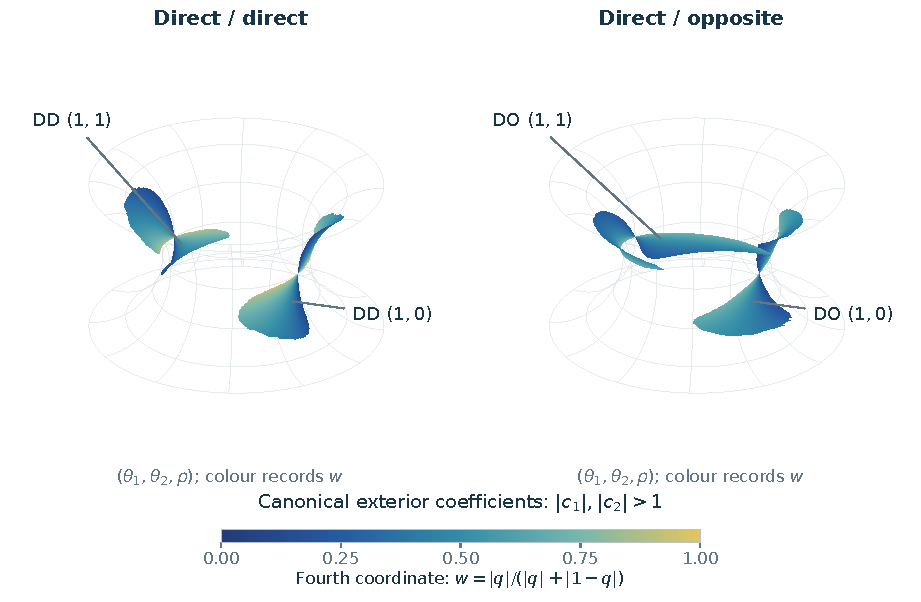
\includegraphics[width=\textwidth]{figures/four_family_projection.pdf}
\caption{Four selected stable slices placed in the four-dimensional
atlas by exterior coefficients $|c_1|,|c_2|>1$ and projected using
\eqref{eq:zipper-three-dimensional-projection}. DD and DO occupy
separate orientation charts. Colour records the fourth coordinate
$w$; the visible sheets consist of certified stable parameter cells.
The wireframe is the outer reference $\rho=2$. Position alone omits
$w$, and the imposed toroidal opening has no implication for the
topology of the connectedness locus. The canonical DO phase rotation
is included as in~\eqref{eq:four-exterior-surfaces}.}
\label{fig:zipper-stable-atlas}
\end{figure}

\begin{figure}[p]
\centering
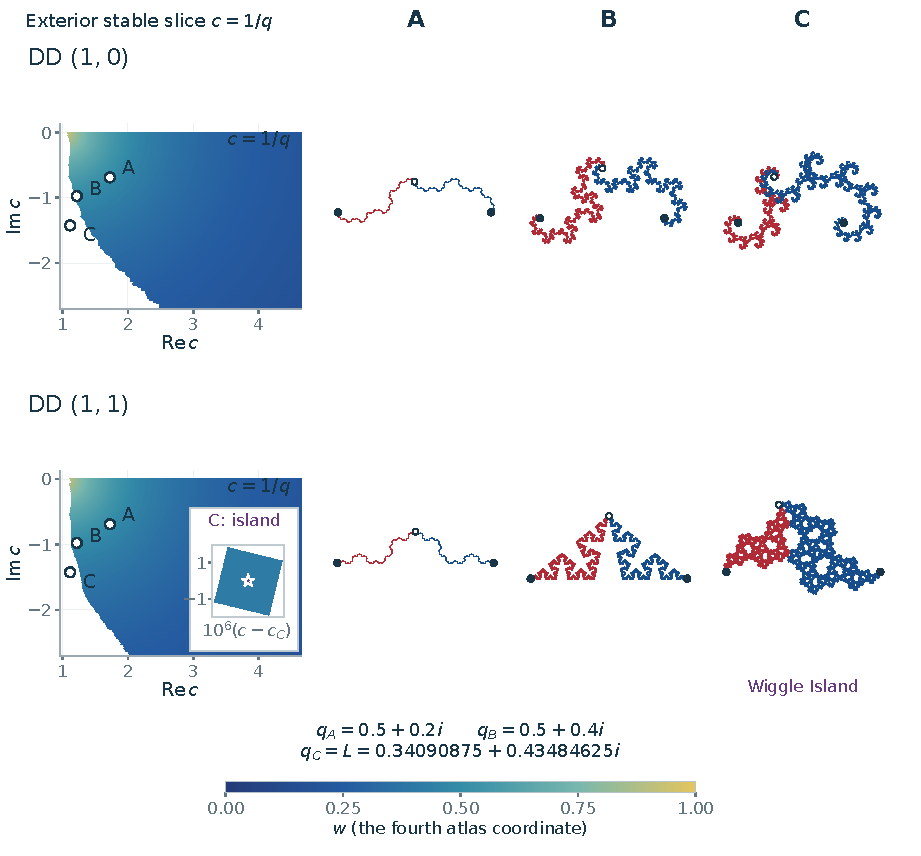
\includegraphics[width=\textwidth]{figures/four_family_DD.pdf}
\caption{DD$(1,0)$ and DD$(1,1)$: certified stable inner covers in the
unsigned endpoint coordinate $c=1/q$, linked to the three common
curve probes~\eqref{eq:three-shared-zipper-probes}. The corresponding
canonical exterior coordinates are $c_1=-c$ and
$c_2=(-1)^{e_2}c/(c-1)$. The DD$(0,1)$ reflection is represented
by DD$(1,0)$. Red and blue distinguish the first-level curve pieces;
they are not membership labels. The tiny certified DD$(1,1)$
neighbourhood of $L$ is shown separately from the common-scale cover.
The curve approximations and their error bounds are recorded in
Appendix~\ref{app:zipper-computation}.}
\label{fig:zipper-dd-gallery}
\end{figure}

\begin{figure}[p]
\centering
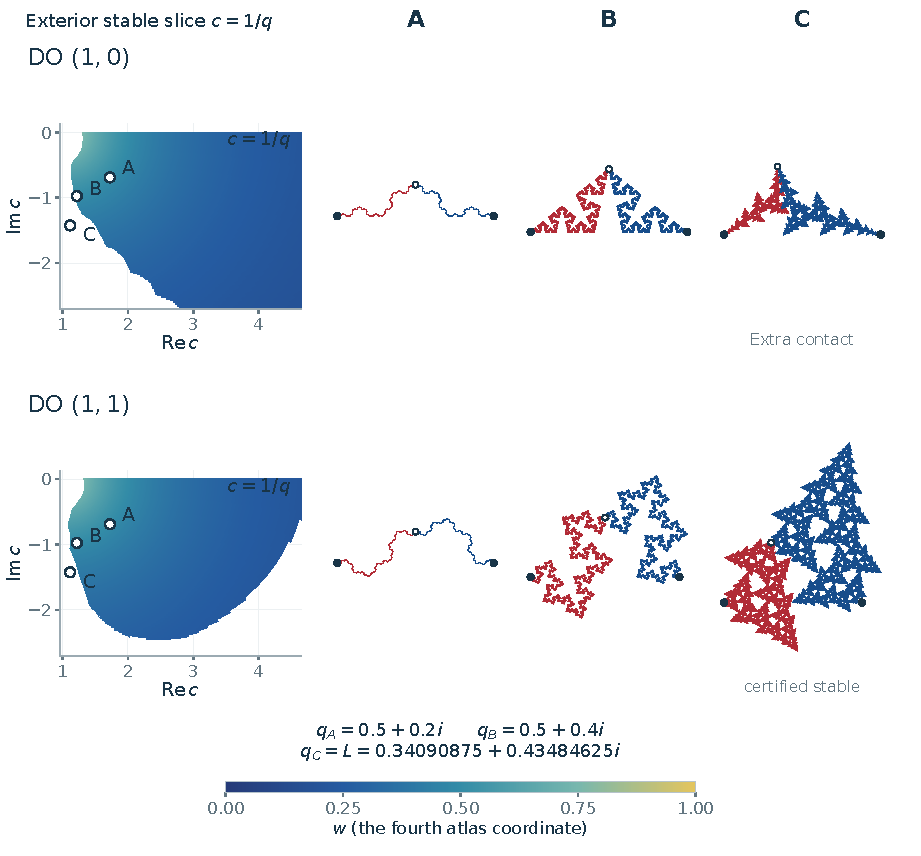
\includegraphics[width=\textwidth]{figures/four_family_DO.pdf}
\caption{DO$(1,0)$ and DO$(1,1)$ at the same exterior slice coordinates
and curve probes as Figure~\ref{fig:zipper-dd-gallery}. The opposite
map contributes the phase factor $N/\overline N$ in the canonical
exterior coefficient $c_2$. The painted slice regions certify stable
parameters. The common probe $q_C=L$ produces an additional
identification for DO$(1,0)$ and an embedded curve for DO$(1,1)$;
these conclusions come from certificates, independently of the
finite curve drawings.}
\label{fig:zipper-do-gallery}
\end{figure}
